%*******10********20********30********40********50********60********70********80
\clearpage

\subsection{Result And Discussion}

In this section, the relationship between concrete's behavior of expansion and its losses on mechanical properties are discussed.

By RBSM, all information of the 3-dimensional cracking behavior can be recorded and analysis numerically. While it is with difficulties to summarized the behavior of expansion by the naked eye, all stress distribution and crack generation process are able to be analyzed numerically.

For example, in Figure \ref{fig:Total_Number_of_Cracks}, the relationship of total cracked interfaces and its relationship with residual compressive strength (in a ratio of the compressive strength of undamaged model) is presented.

It can be seen that as the total cracking interfaces number increase, the residual compressive strength decrease in all kinds of expansion applied.

\begin{figure}[ht!]
\centering
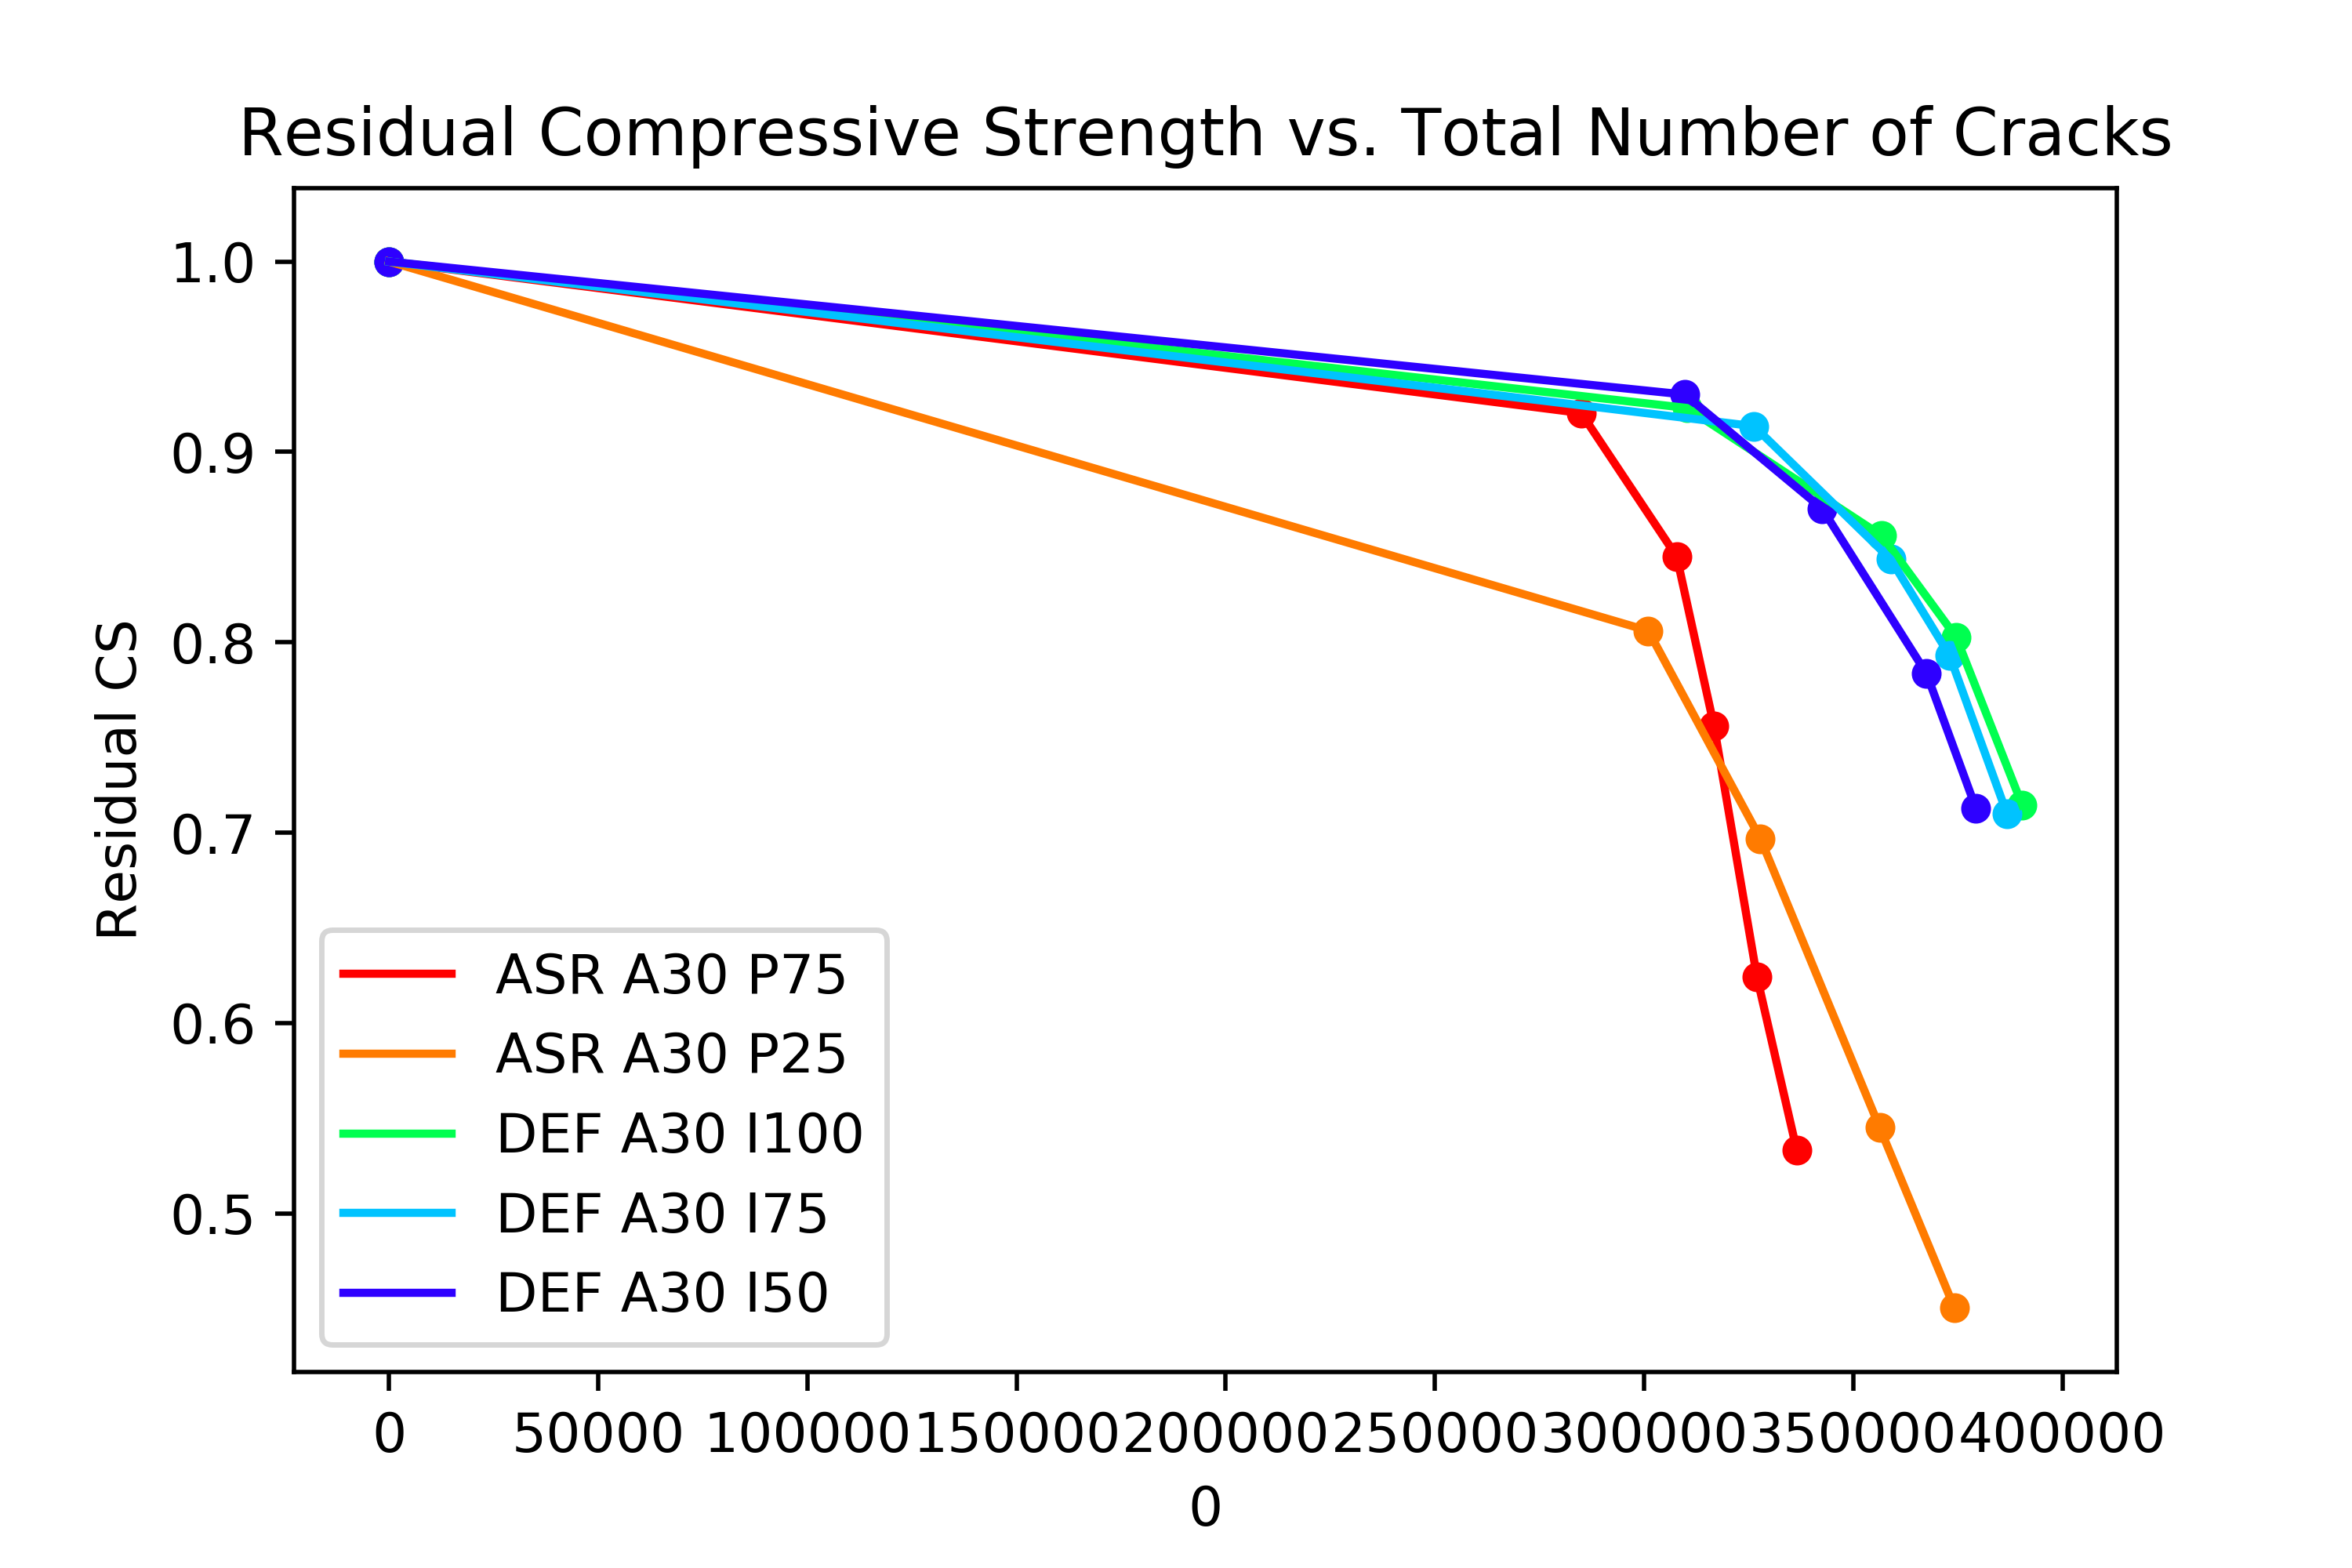
\includegraphics[width=.8\linewidth]{Files/exp_3D/Residual_Compressive_Strength_vs_Total_Number_of_Cracks.png}
  \caption{Residual Compressive Strength vs. Total Number of Cracks}
  \label{fig:Total_Number_of_Cracks}
\end{figure}

While structually, larger crack in width do represent larger damage, especially in its mechanical properties, here in Figure \ref{fig:Total_Number_of_Cracks_0.0005+} the relationship between total number of cracked interfaces larger than 0.0005 mm and the residual compressive strength is plotted.

This time clear linear relationship between the number of cracks larger than 0.0005 mm and the reducing in its compressive strength can be seen here, both in ASR expansion and DEF expansion.

\begin{figure}[ht!]
\centering
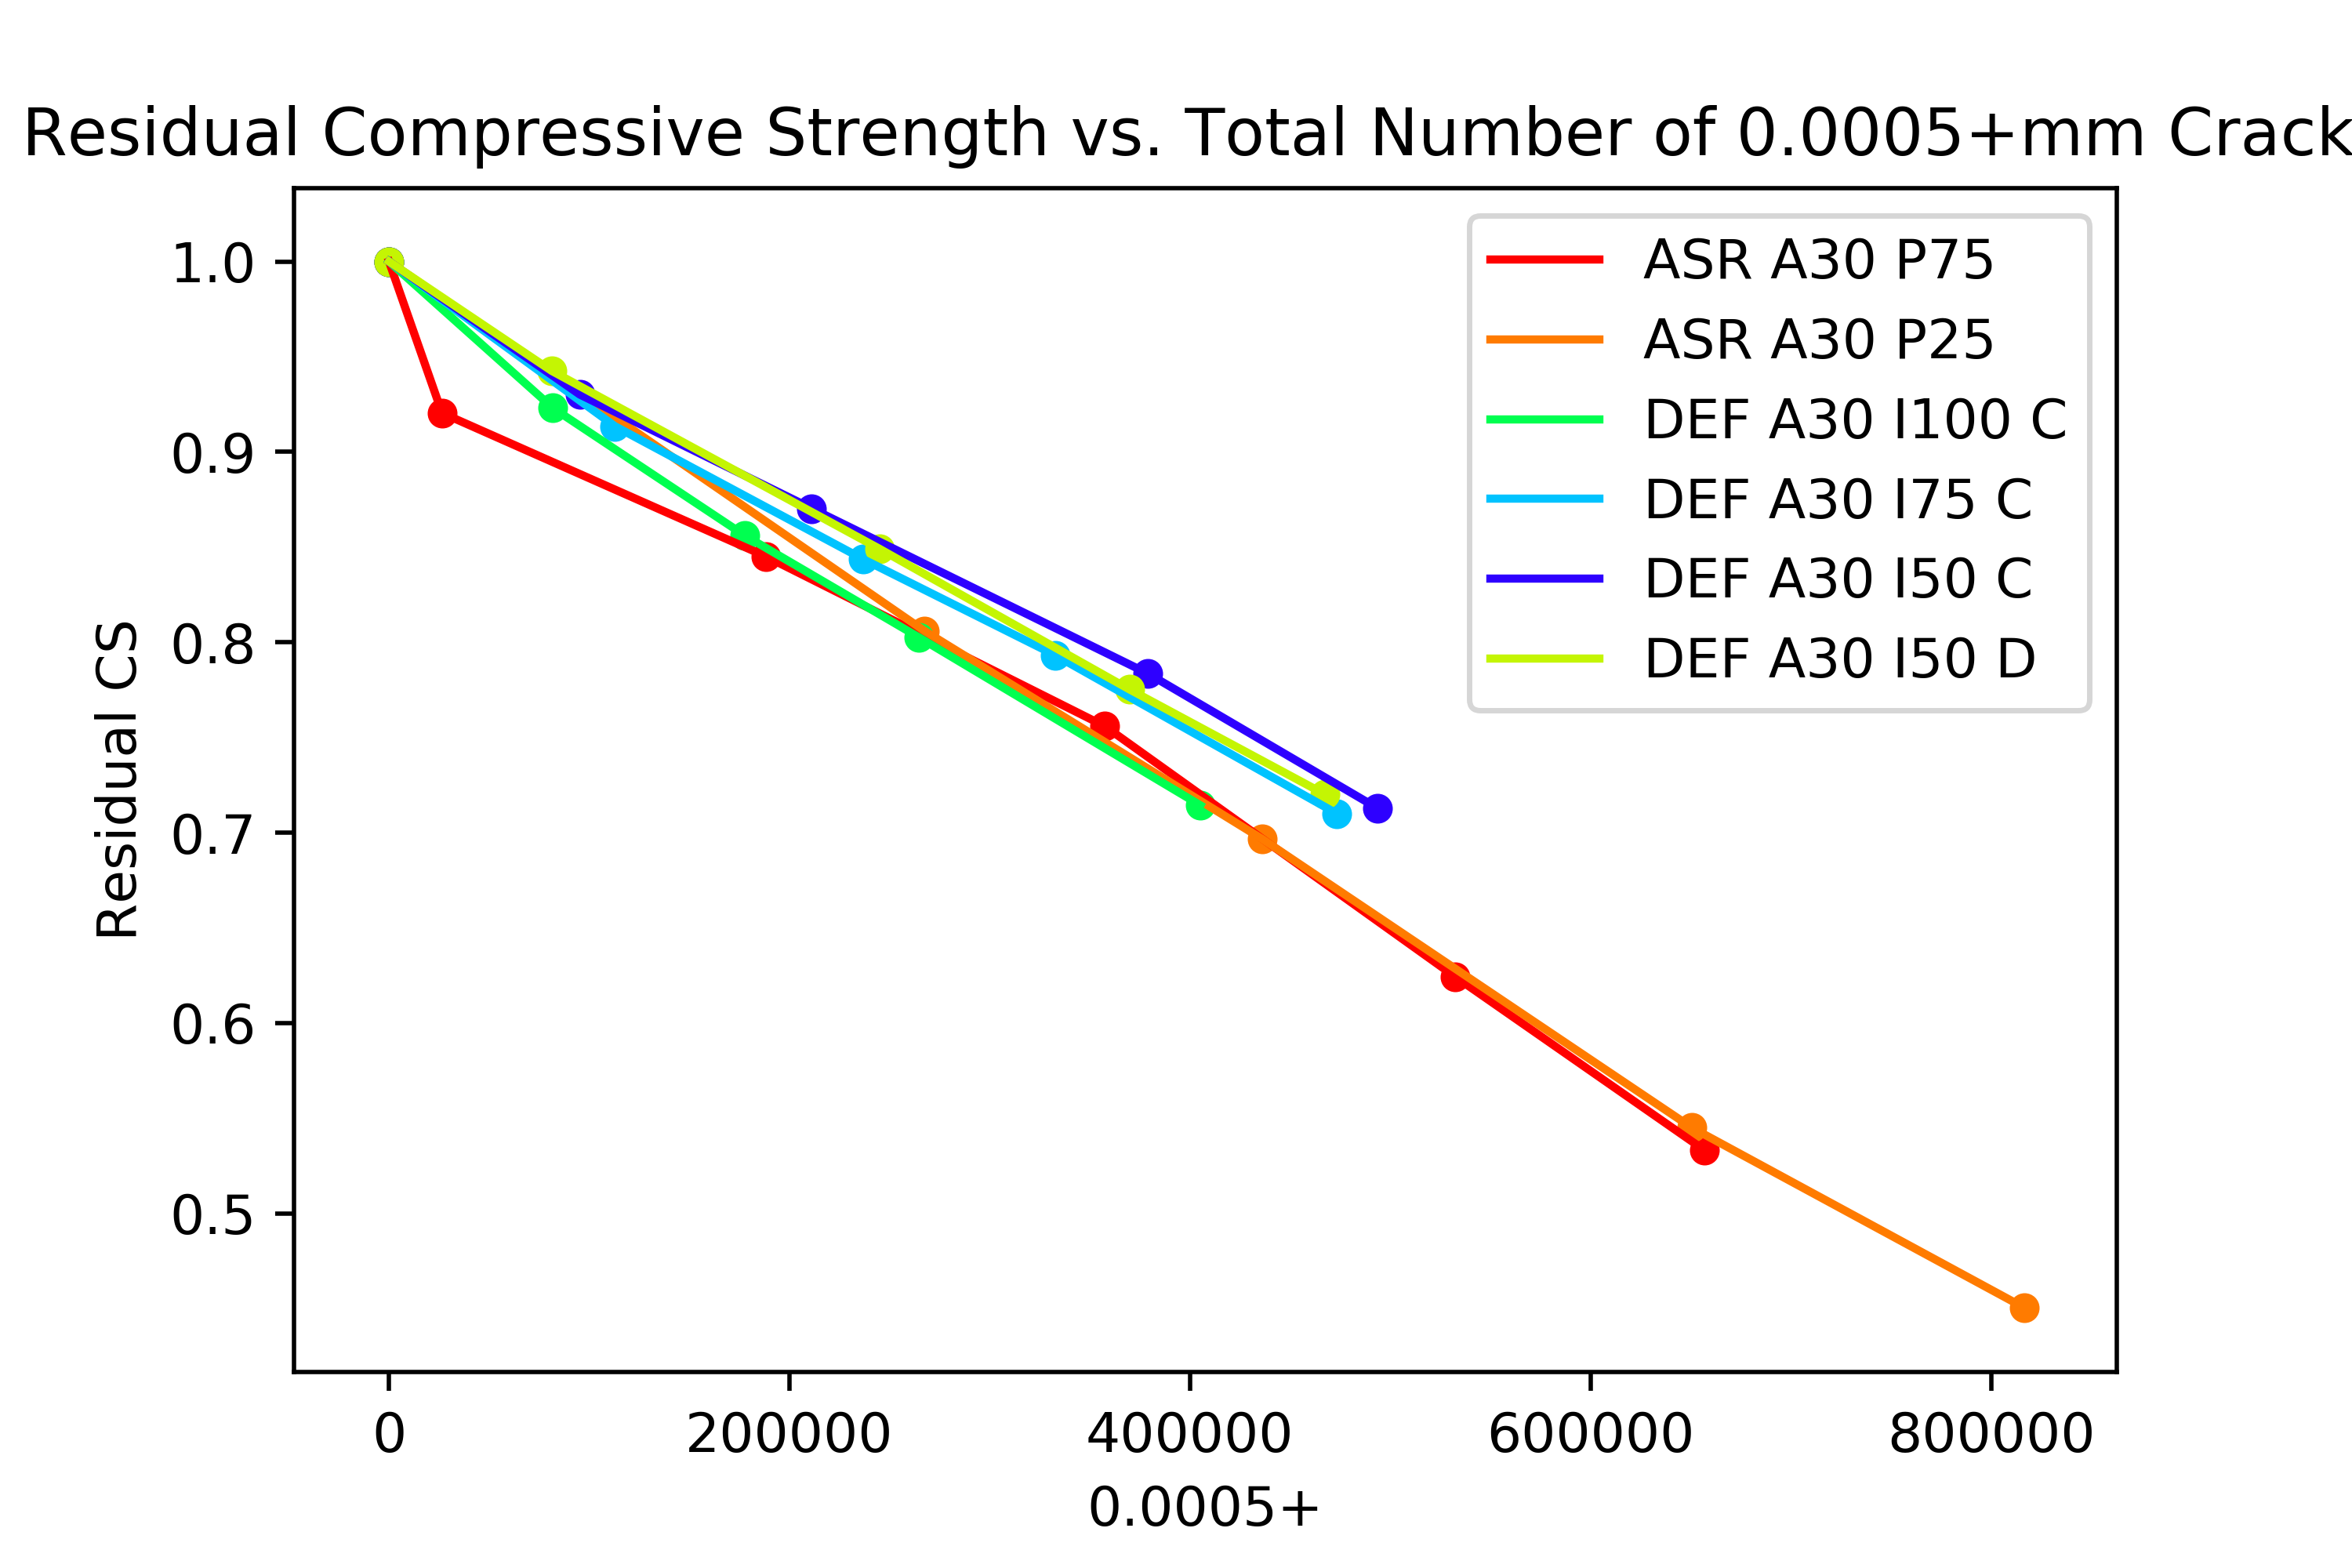
\includegraphics[width=.8\linewidth]{Files/exp_3D/Residual_Compressive_Strength_vs_Total_Number_of_0005_Cracks.png}
  \caption{Residual Compressive Strength vs. Total Number of Cracks over 0.0005 mm}
  \label{fig:Total_Number_of_Cracks_0.0005+}
\end{figure}

If plot the total number of cracked interfaces larger than 0.001 mm and the residual compressive strength, as shown in Figure \ref{fig:Total_Number_of_Cracks_0.001+}, similar trand is shown, indicate that the number of wider cracks largely determined the residual compressively strength.
\begin{figure}[ht!]
\centering
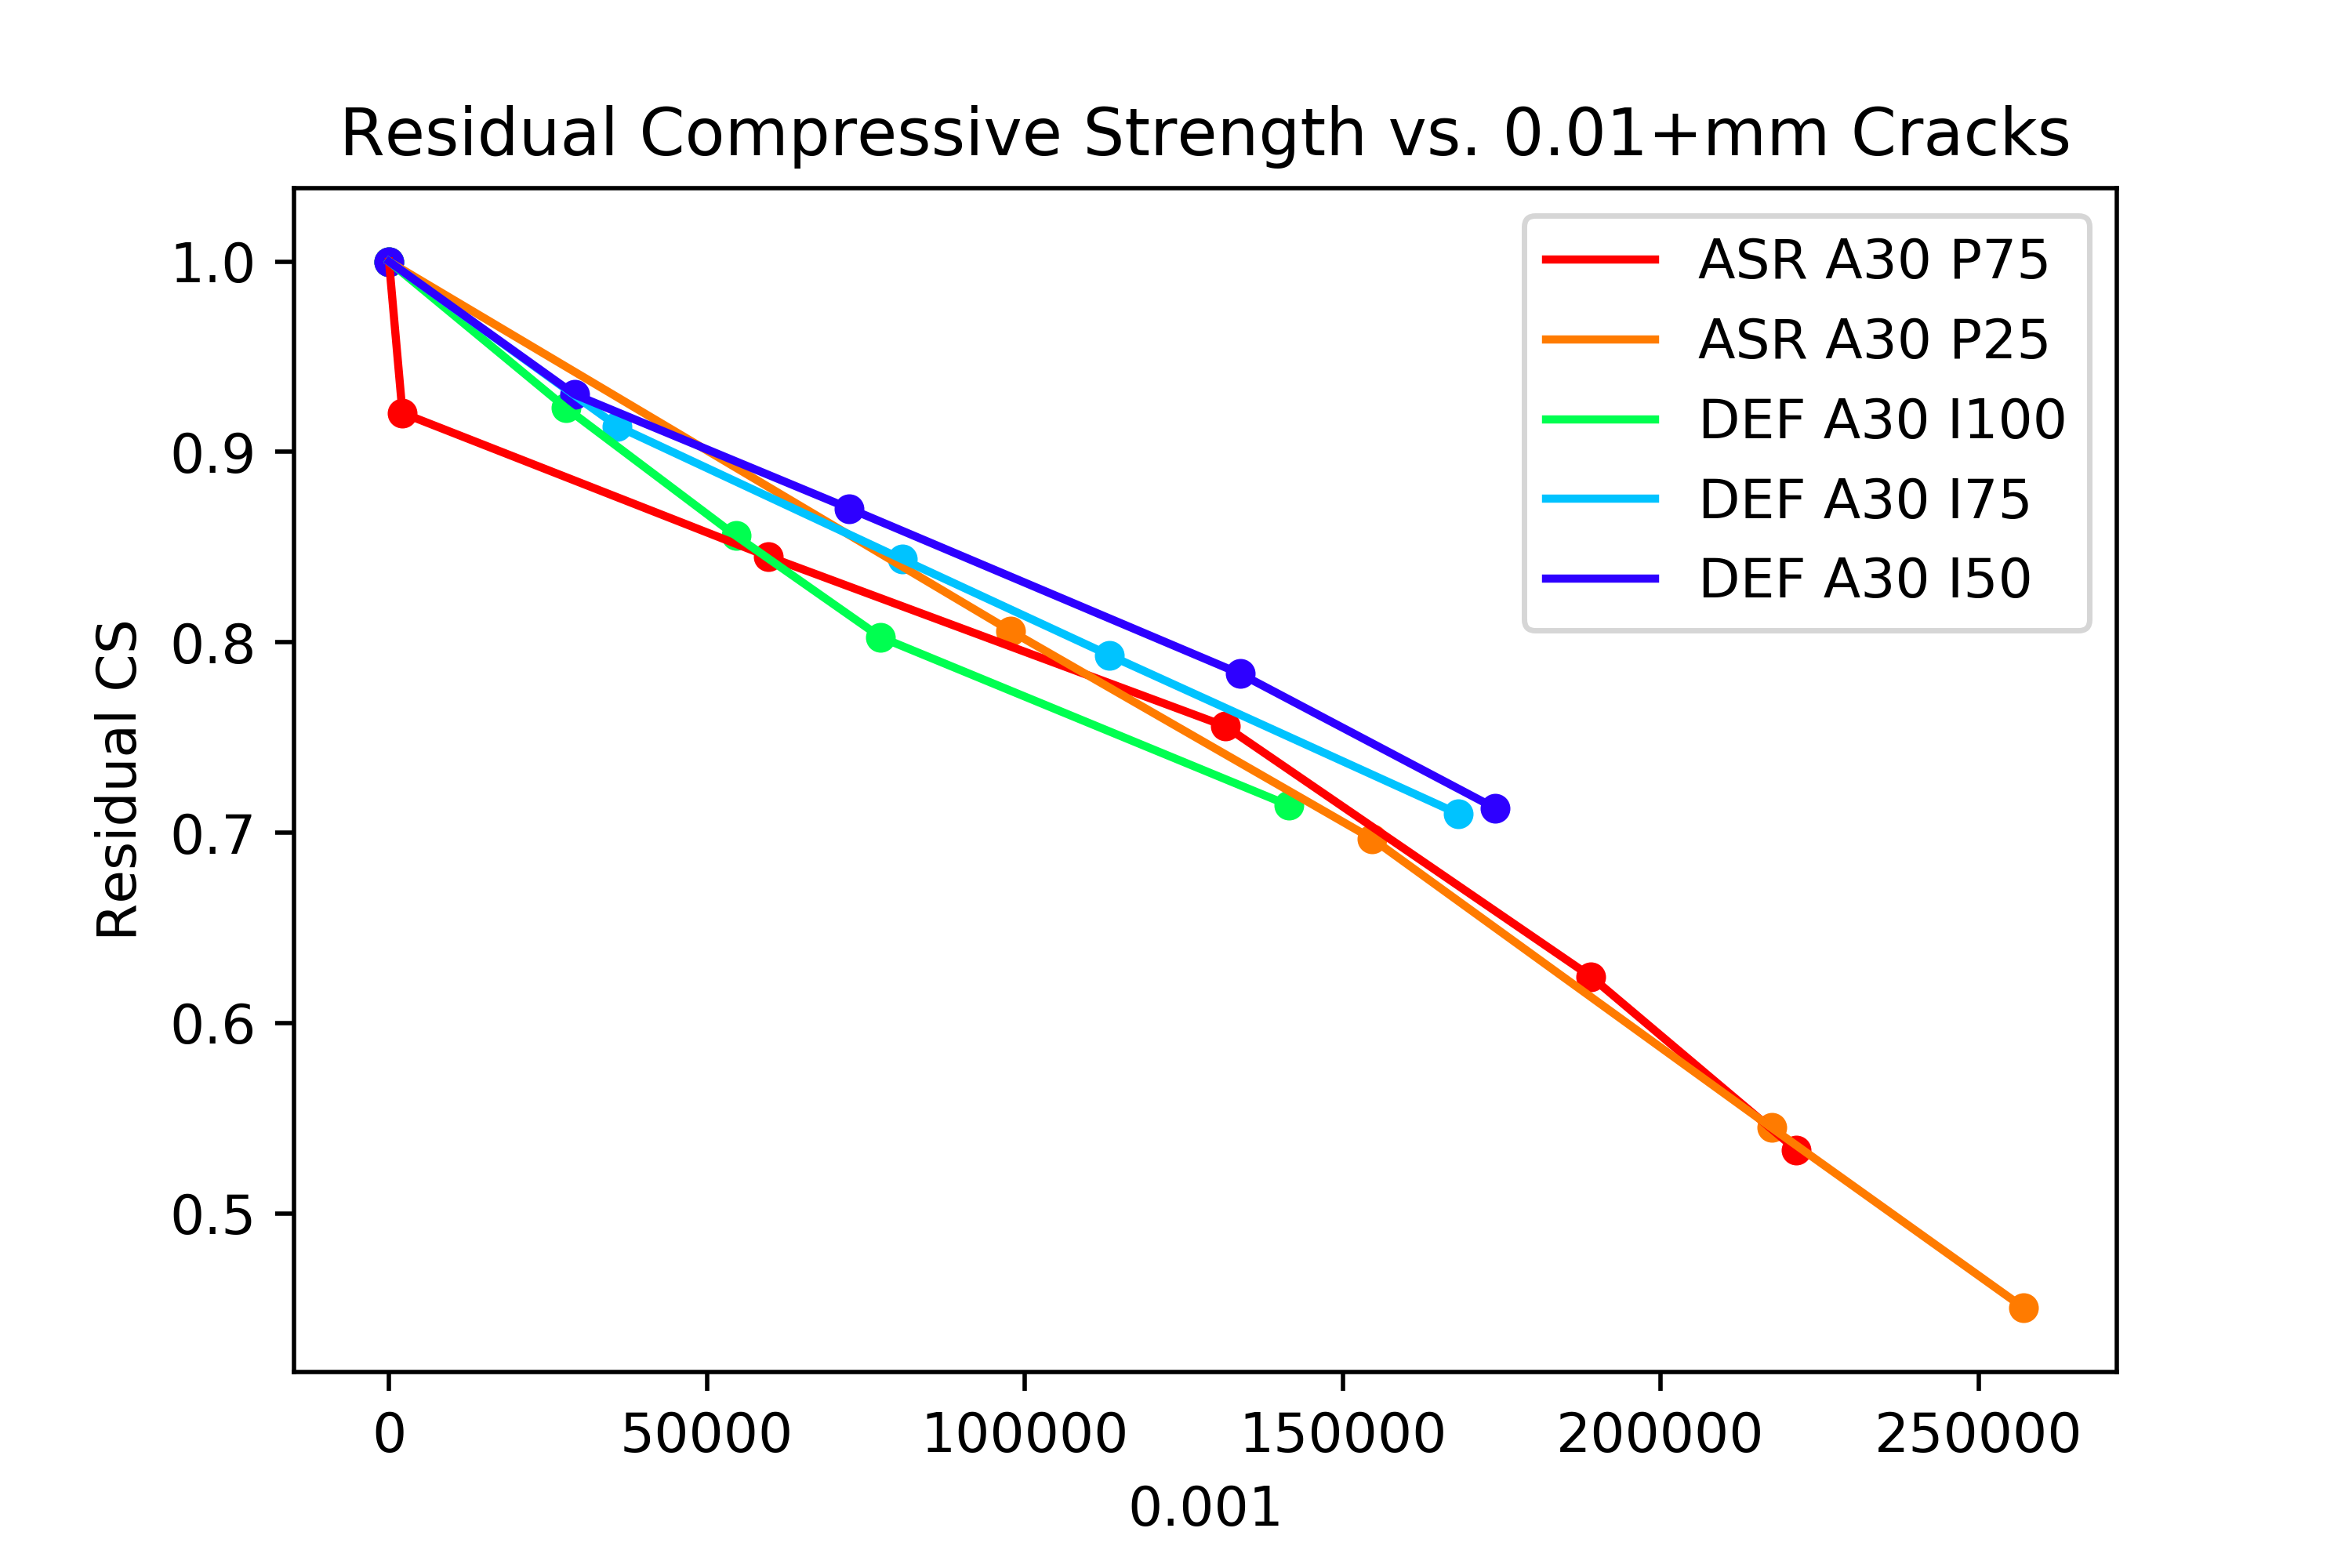
\includegraphics[width=.8\linewidth]{Files/exp_3D/Residual_Compressive_Strength_vs_Total_Number_of_001_Cracks.png}
  \caption{Residual Compressive Strength vs. Total Number of Cracks over 0.001 mm}
  \label{fig:Total_Number_of_Cracks_0.001+}
\end{figure}

While if plotting the total number of cracked interfaces relately smaller and the residual compressive strength, the linear corrisbonding relationship does not show up, and shown in Figure \ref{fig:c1}, Figure \ref{fig:c2}, and Figure \ref{fig:c3}. This result indicte that the residual compressive strength is less depends on smaller scale cracks comparing to the larger cracks.

\begin{figure}[ht!]
\centering
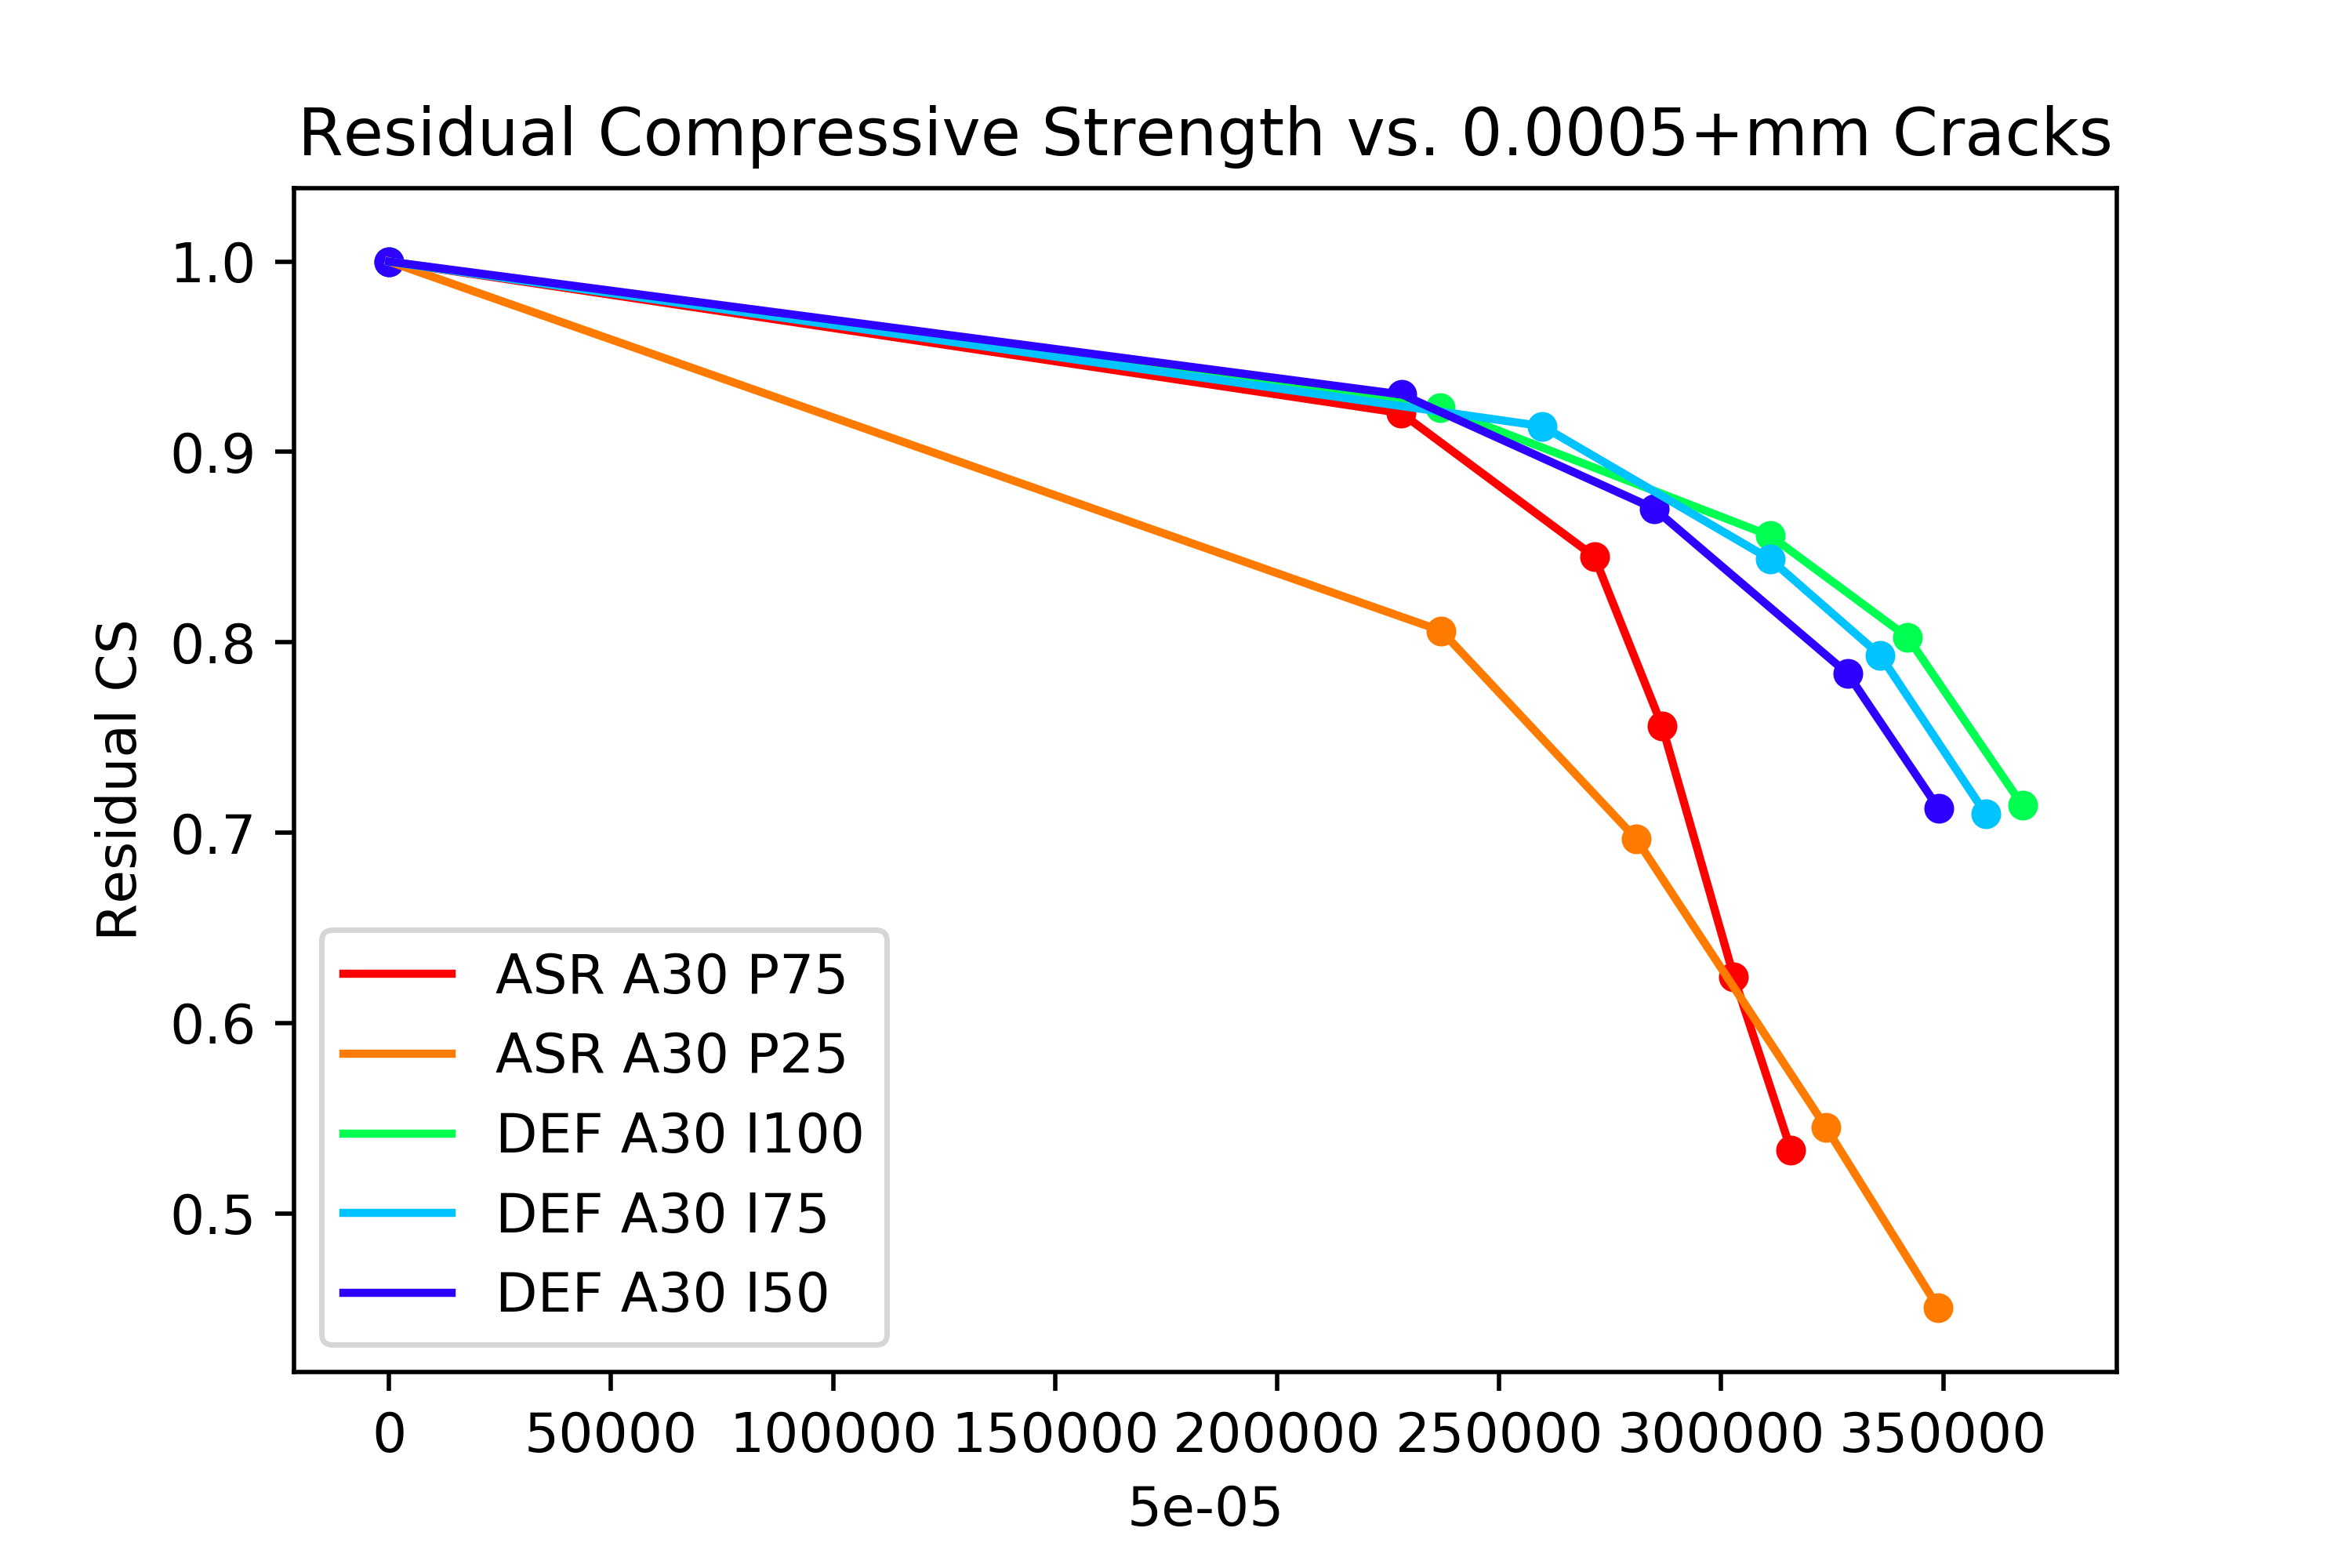
\includegraphics[width=.8\linewidth]{Files/exp_3D/1.png}
  \caption{Residual Compressive Strength vs. Total Number of 0.0005+mm Cracks}
  \label{fig:c1}
\end{figure}

\begin{figure}[ht!]
\centering
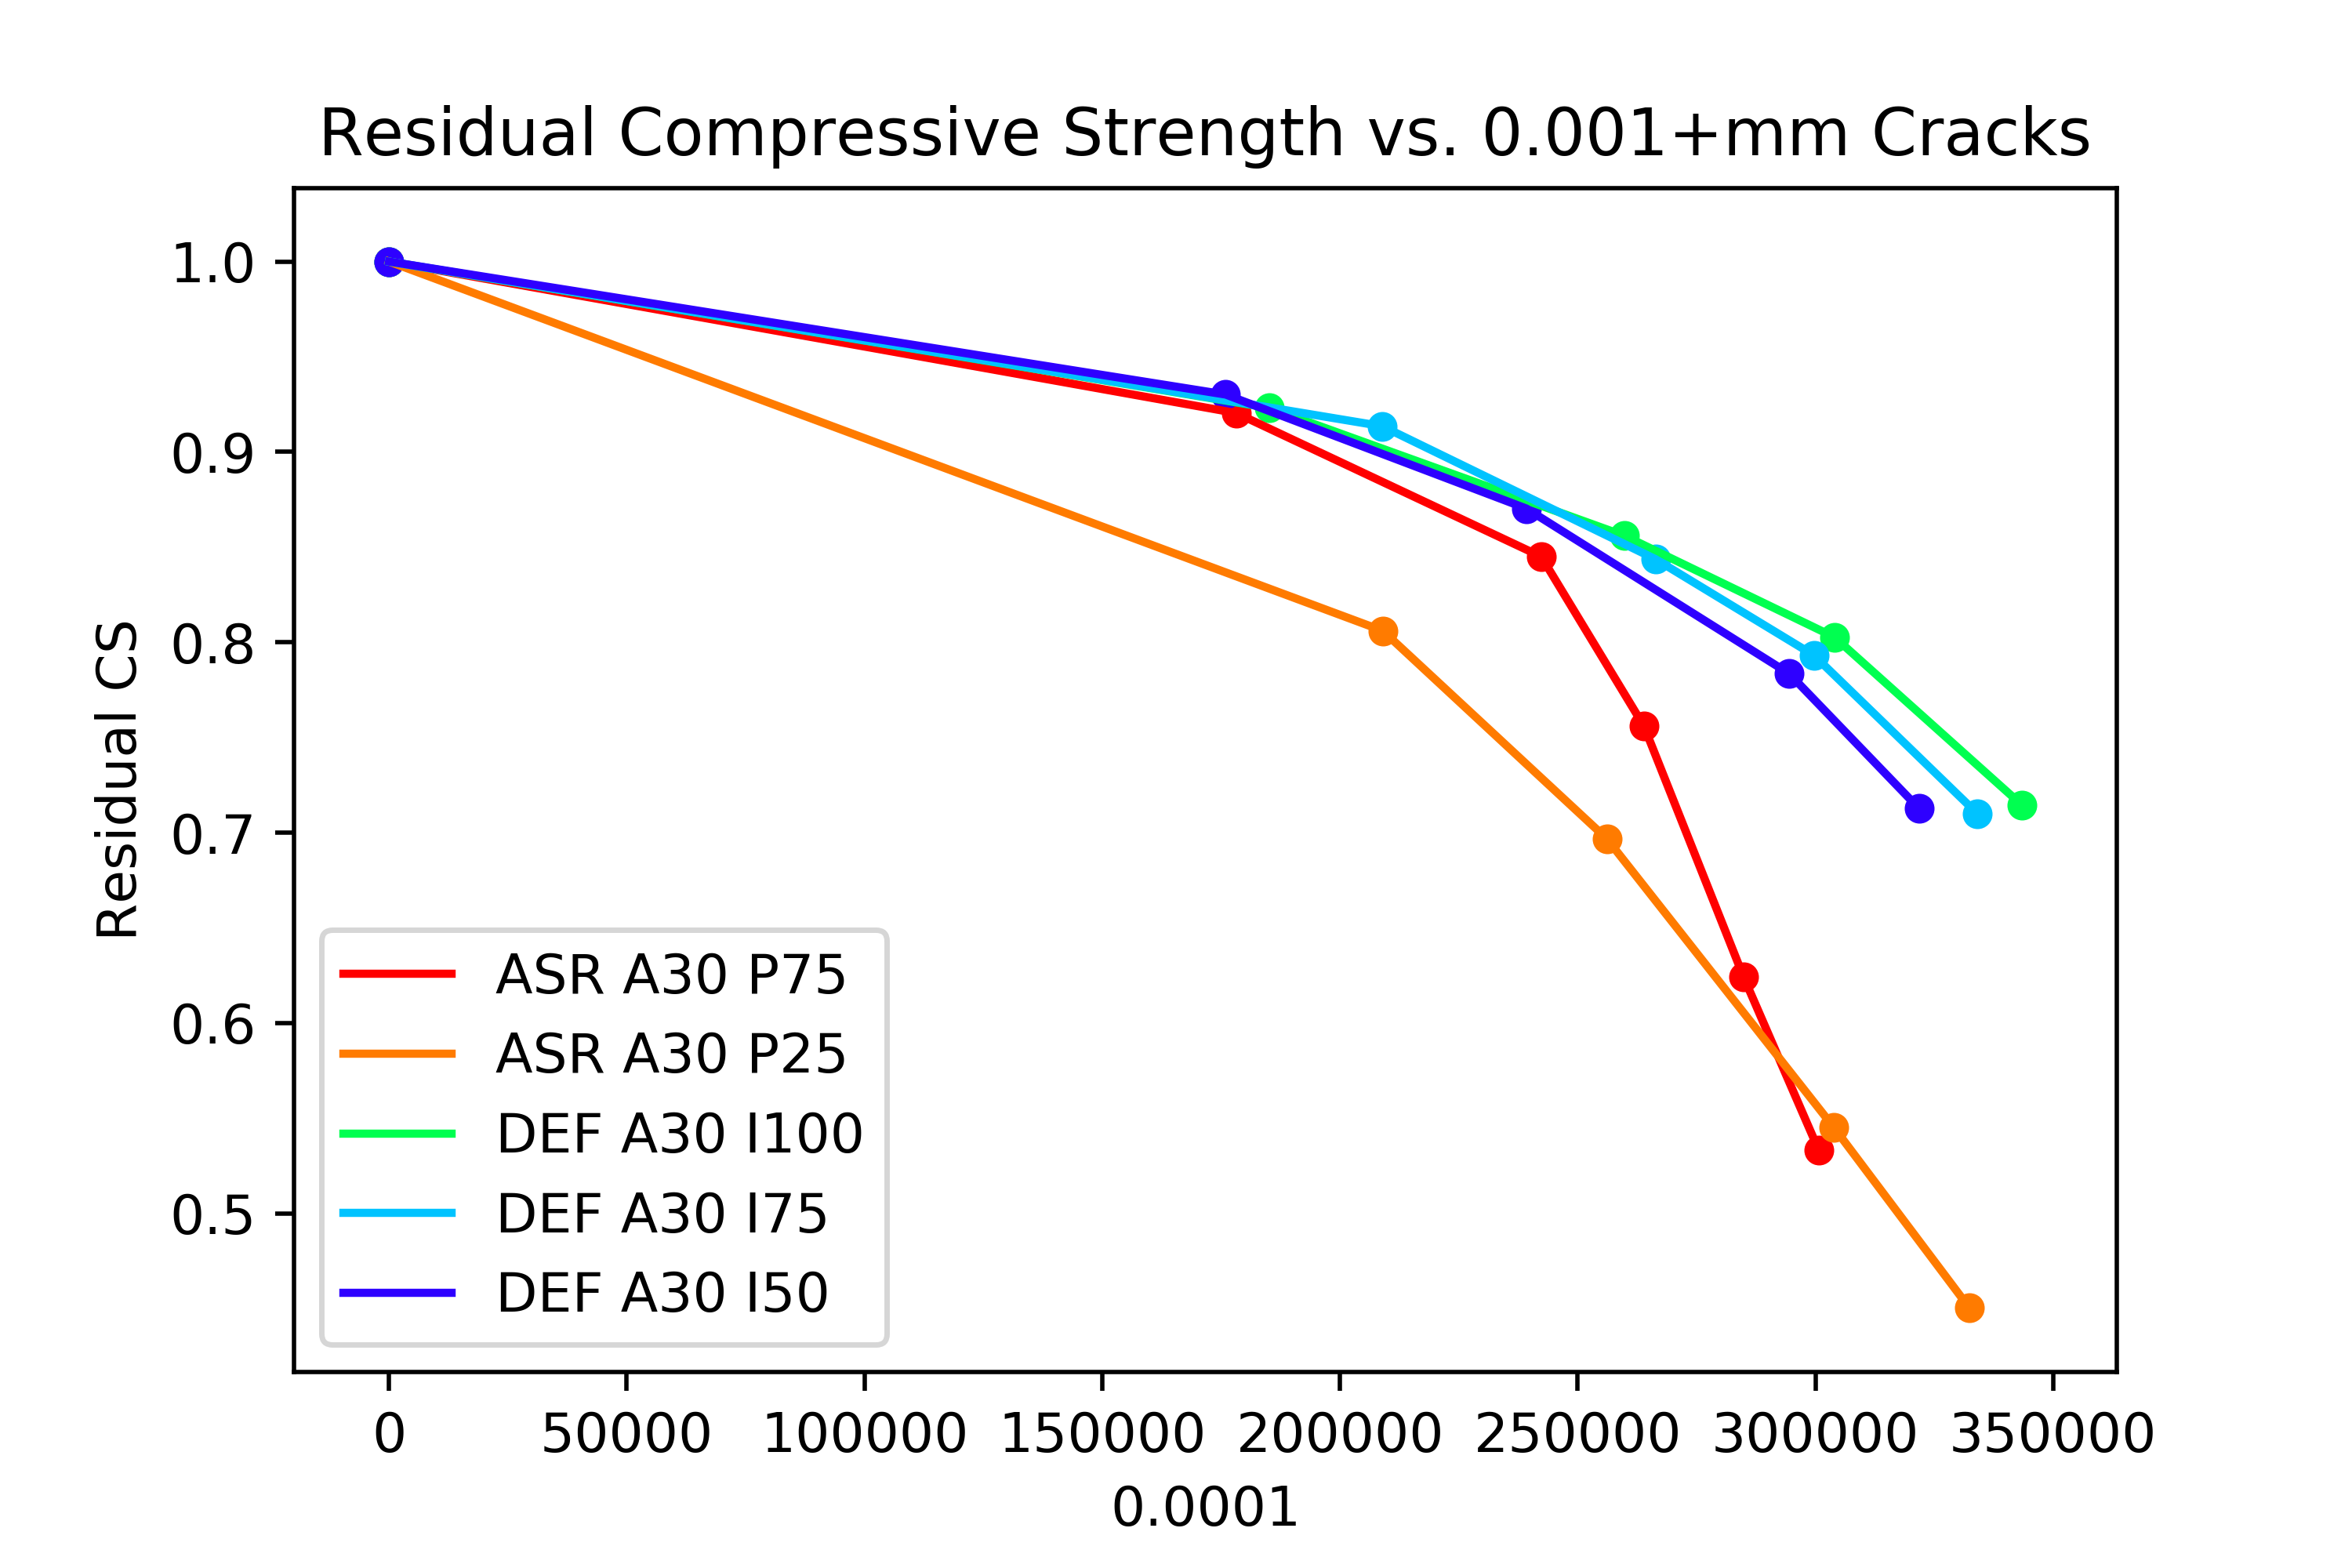
\includegraphics[width=.8\linewidth]{Files/exp_3D/2.png}
  \caption{Residual Compressive Strength vs. Total Number of 0.001+mm Cracks}
  \label{fig:c2}
\end{figure}

\begin{figure}[ht!]
\centering
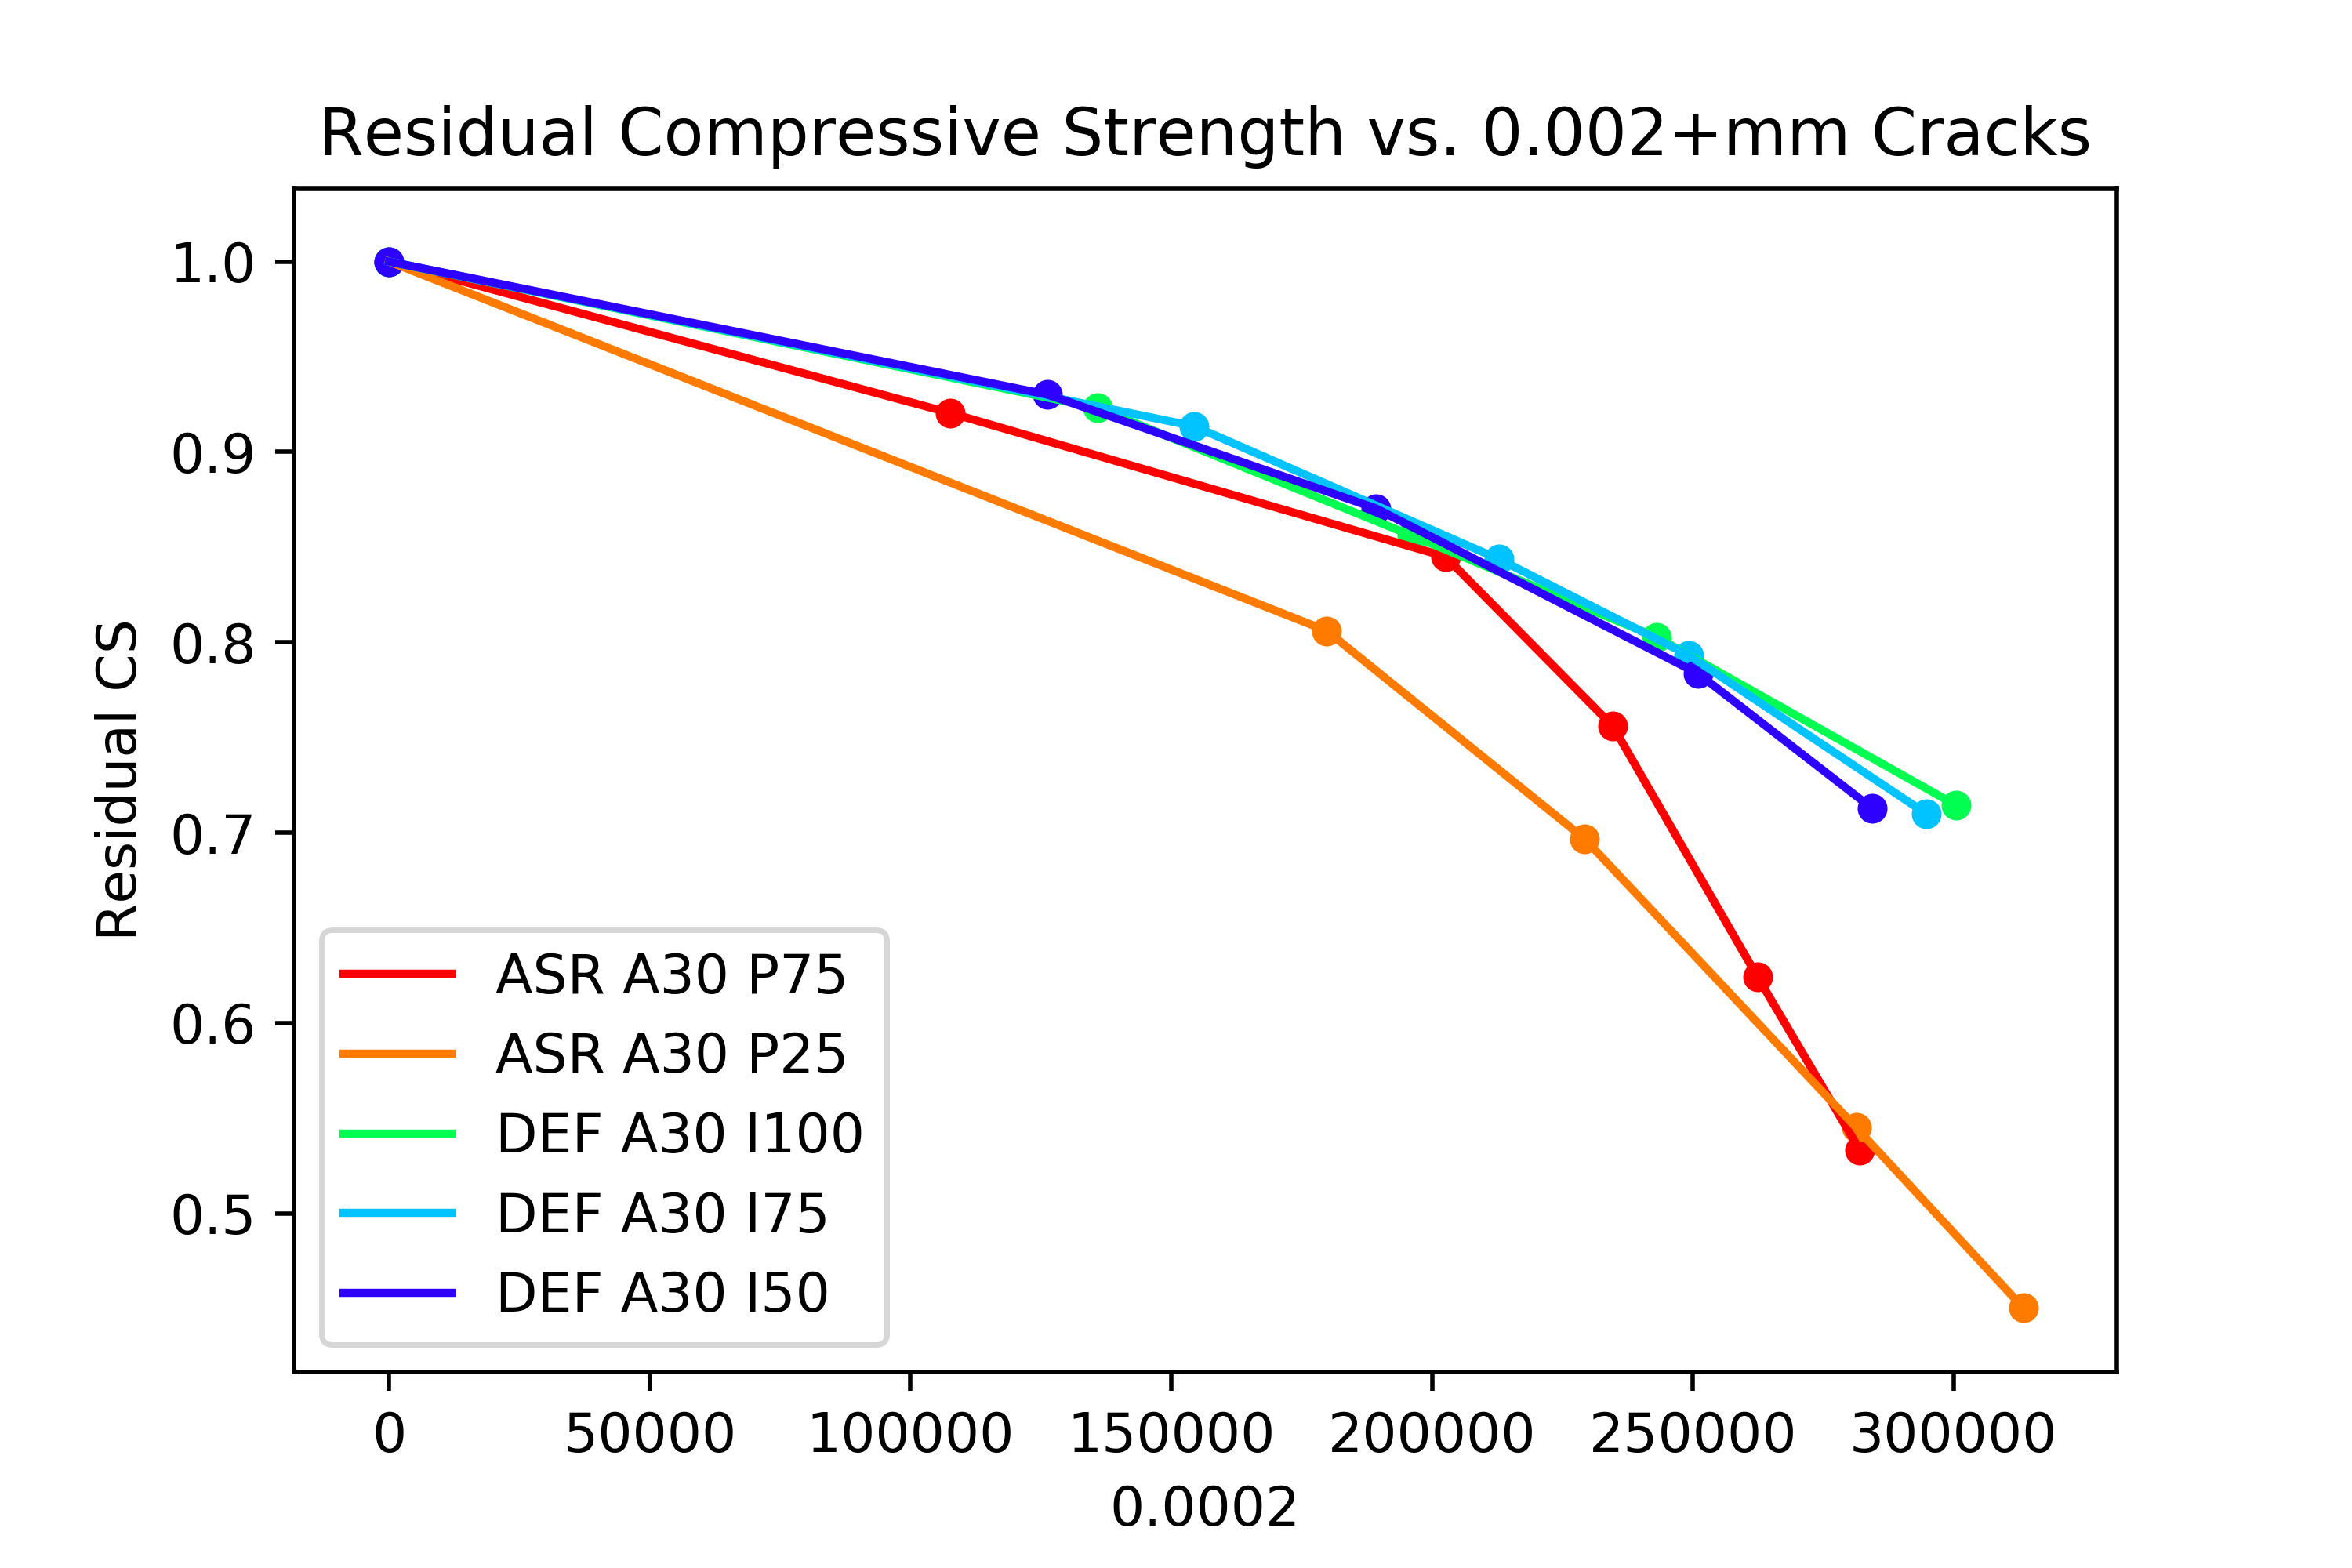
\includegraphics[width=.8\linewidth]{Files/exp_3D/3.png}
  \caption{Residual Compressive Strength vs. Total Number of 0.002+mm Cracks}
  \label{fig:c3}
\end{figure}


This result implied that while the expansion mechanism and cracking pattern can be different in ASR and DEF expansion, the residual mechanical properties, for example, the compressive strength, is determined by the existence of larger cracks (0.005 mm+ here). This may offer us a new direction in the analysis the residual capacity of the expanded concrete structure.

The relationship found here also explained the reason of differences in loss of mechanical properties when same global scale expansion applied by different mechanisms. As the cracking pattern caused by ASR and DEF are different, shown in Figure \ref{fig:expcs}, their mechanical properties loss in same expansion can be different.

At same one-dimensional global expansion, shown in Figure \ref{fig:ASR_A30P75_3_3Dsss} and Table \ref{table:ASRs_30_EXP}, ASR expanded models have more larger cracks, while cracks causes by DEF are relately concentrated in smaller width range. As the result, in our simulation, ASR have less residual compressive strength comparing to DEF cases.

\begin{figure}[ht!]
\centering
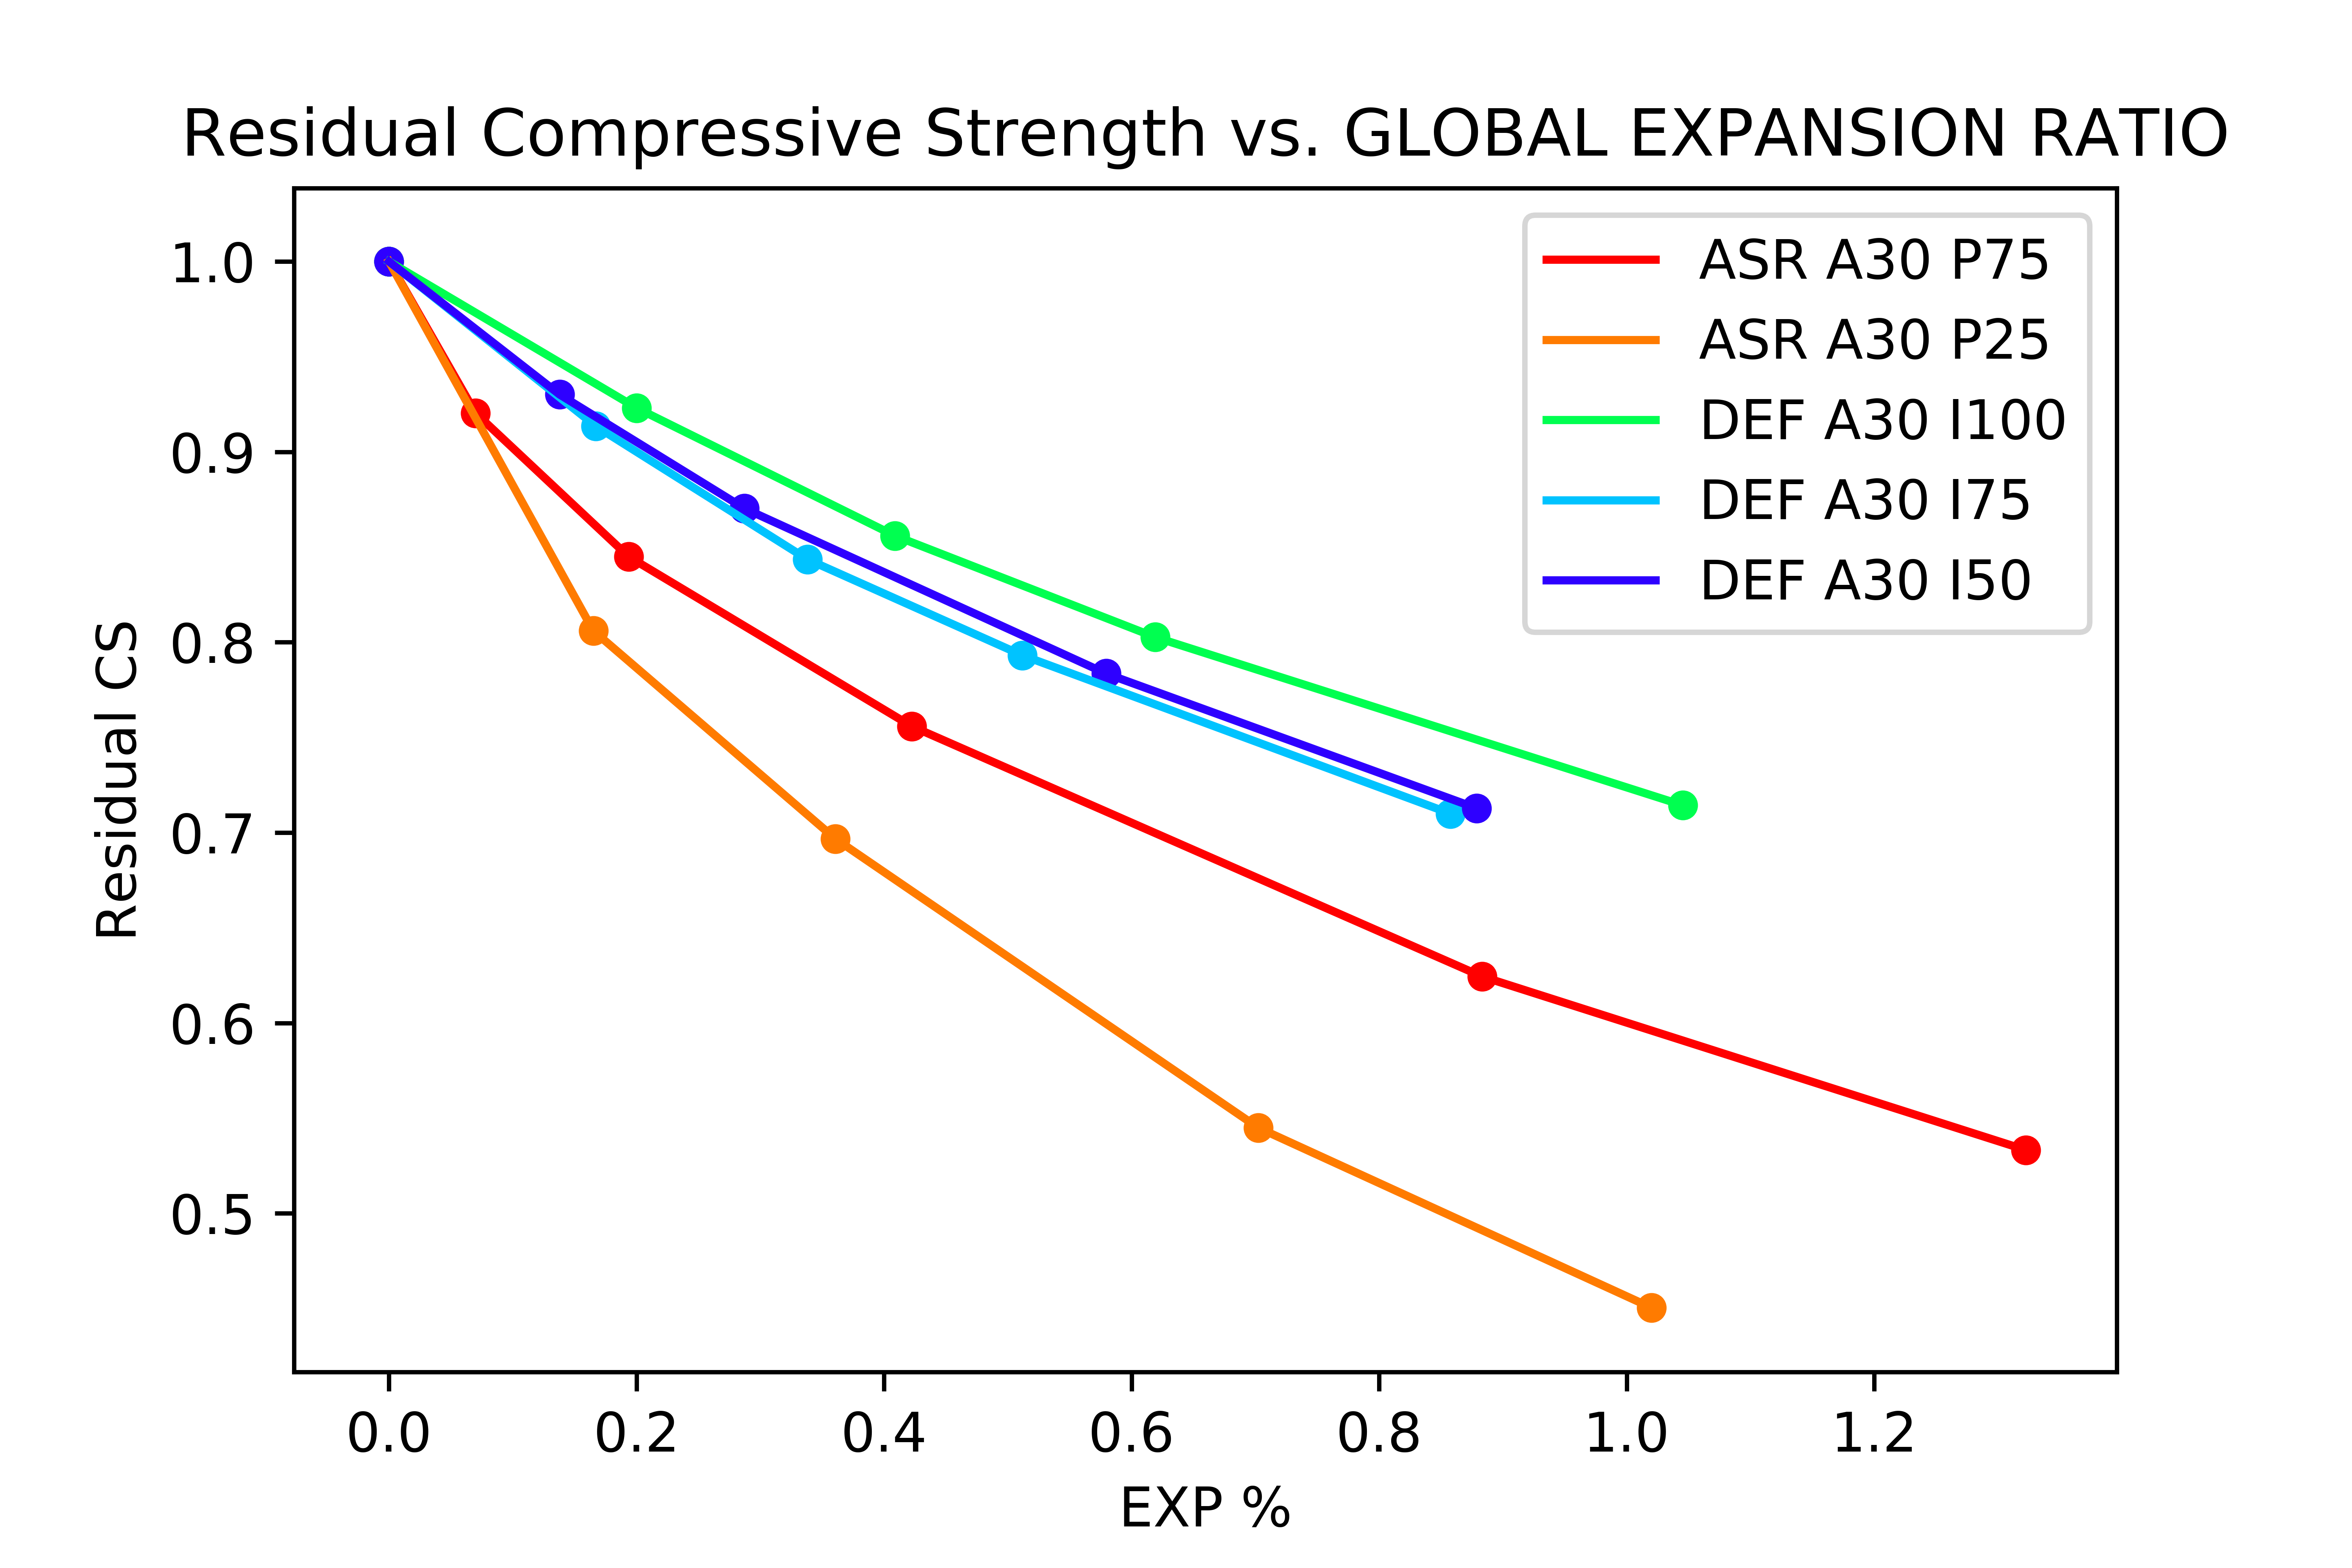
\includegraphics[width=.8\linewidth]{Files/exp_3D/EXPvsCS.png}
  \caption{Residual Compressive Strength vs. Expansion[\%]}
  \label{fig:expcs}
\end{figure}


\begin{figure}[ht!]
\centering
    %*******
    \begin{subfigure}{.33\textwidth}
      \centering
      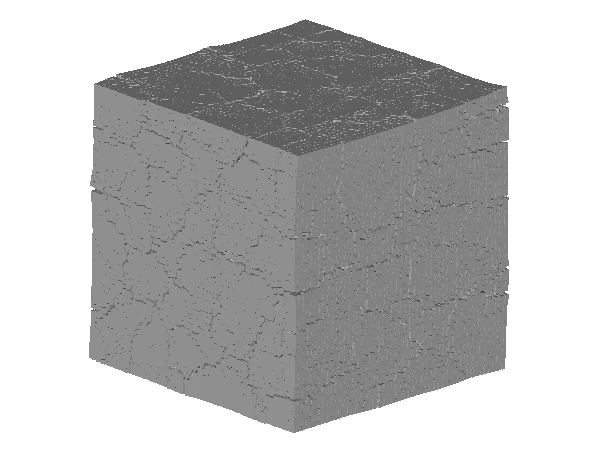
\includegraphics[width=.8\linewidth]{Files/exp_3D/ASR/A30P75_3_3d.png}
    \end{subfigure}%
    %*******
    \begin{subfigure}{.33\textwidth}
      \centering
      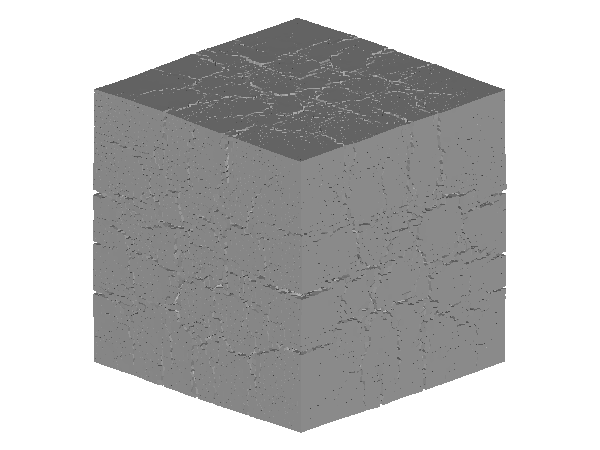
\includegraphics[width=.8\linewidth]{Files/exp_3D/DEF/A30X0C_3_3d.png}
    \end{subfigure}%
    %*******
    \begin{subfigure}{.33\textwidth}
      \centering
      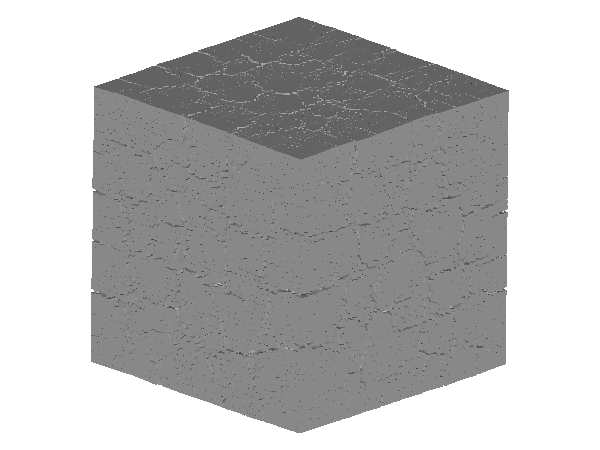
\includegraphics[width=.8\linewidth]{Files/exp_3D/DEF/A30X-5C_3_3d.png}
    \end{subfigure}
    %*******
    %*******
    \begin{subfigure}{.33\textwidth}
      \centering
      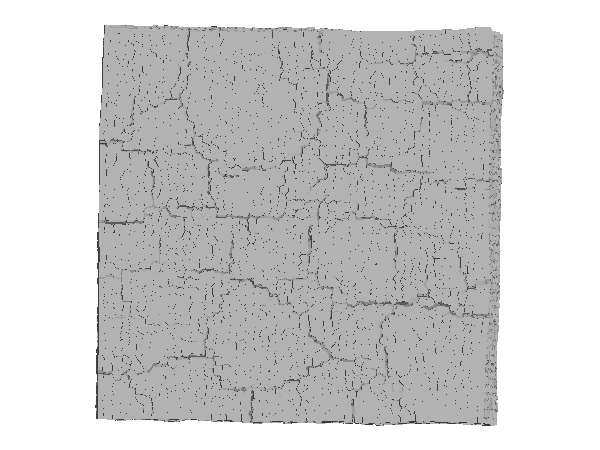
\includegraphics[width=.8\linewidth]{Files/exp_3D/ASR/A30P75_3_3ds.png}
      \caption{ASR A30 P75 Case 3 \\ Surface Crack}
    \end{subfigure}%
    %*******
    \begin{subfigure}{.33\textwidth}
      \centering
      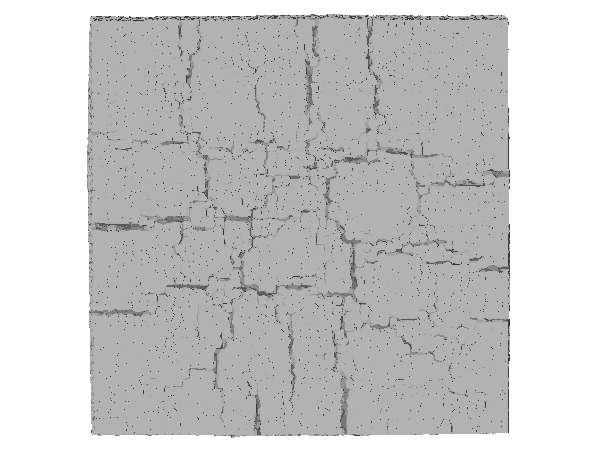
\includegraphics[width=.8\linewidth]{Files/exp_3D/DEF/A30X0C_3_3ds.png}
      \caption{DEF A30 I50 Case 3 \\ Surface Crack}
    \end{subfigure}%
    %*******
    \begin{subfigure}{.33\textwidth}
      \centering
      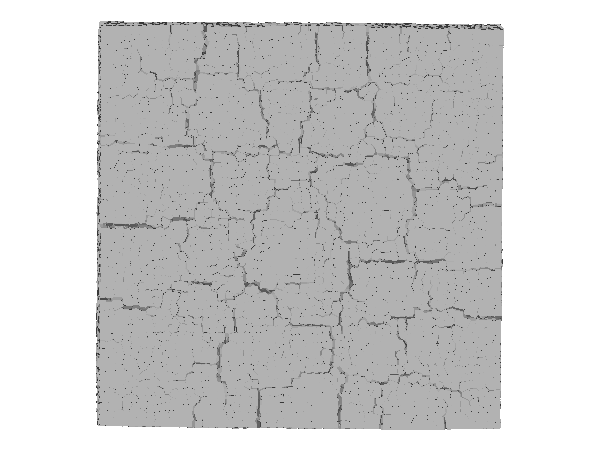
\includegraphics[width=.8\linewidth]{Files/exp_3D/DEF/A30X-5C_3_3ds.png}
      \caption{DEF A30 I75 Case 3 \\ Surface Crack}
    \end{subfigure}
    %*******
    %*******
    \begin{subfigure}{.33\textwidth}
      \centering
      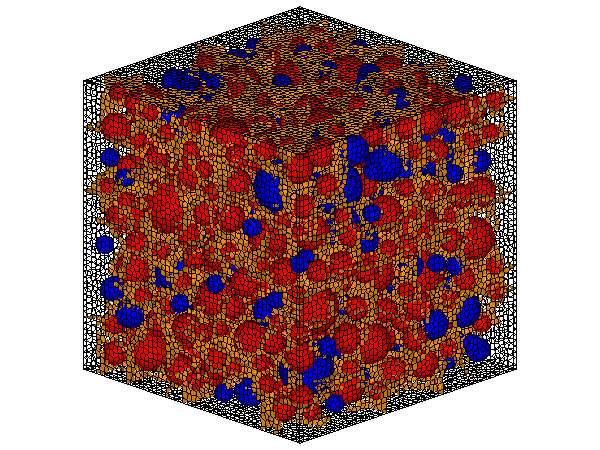
\includegraphics[width=0.8\linewidth]{Files/exp_3D/ASR/A30P75_3_c.png}
      \caption{ASR A30 P75 Case 3 \\ Internal Stress}
    \end{subfigure}%
    %*******
    \begin{subfigure}{.33\textwidth}
      \centering
      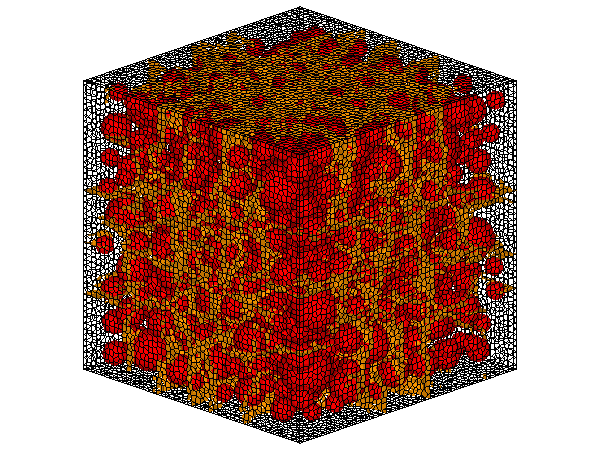
\includegraphics[width=0.8\linewidth]{Files/exp_3D/DEF/A30X0C_3_c.png}
      \caption{DEF A30 I50 Case 3 \\ Internal Stress}
    \end{subfigure}%
    %*******
    \begin{subfigure}{.33\textwidth}
      \centering
      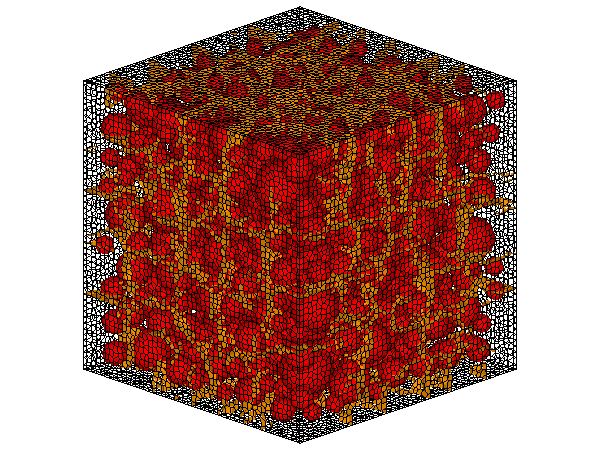
\includegraphics[width=0.8\linewidth]{Files/exp_3D/DEF/A30X-5C_3_c.png}
      \caption{DEF A30 I75 Case 3 \\ Internal Stress}
    \end{subfigure}
    %*******
    %*******
    \begin{subfigure}{.33\textwidth}
      \centering
      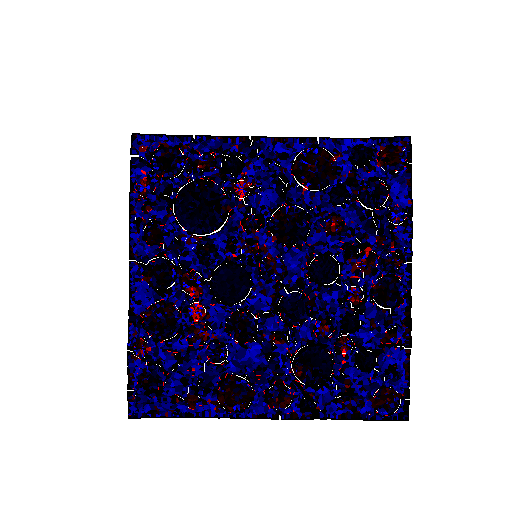
\includegraphics[width=1.0\linewidth]{Files/exp_3D/ASR/A30P75_3_stress.png}
      \caption{ASR A30 P75 Case 3 \\ Internal Stress}
    \end{subfigure}%
    %*******
    \begin{subfigure}{.33\textwidth}
      \centering
      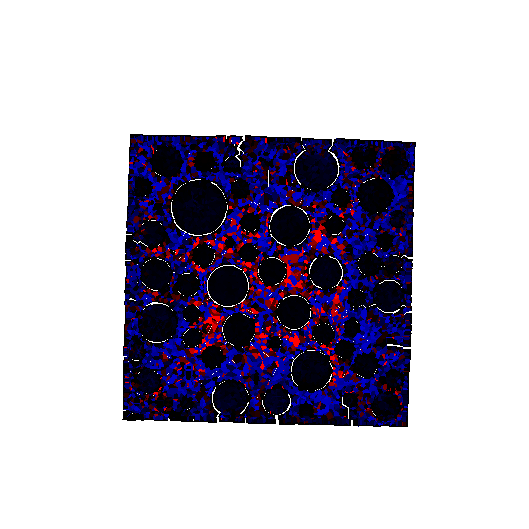
\includegraphics[width=1.0\linewidth]{Files/exp_3D/DEF/A30X0C_3_stress.png}
      \caption{DEF A30 I50 Case 3 \\ Internal Stress}
    \end{subfigure}%
    %*******
    \begin{subfigure}{.33\textwidth}
      \centering
      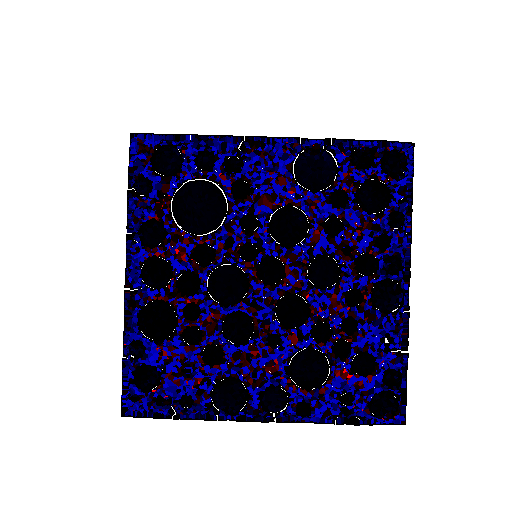
\includegraphics[width=1.0\linewidth]{Files/exp_3D/DEF/A30X-5C_3_stress.png}
      \caption{DEF A30 I75 Case 3 \\ Internal Stress}
    \end{subfigure}
    %*******
  \caption{Cracking Pattern Compare}
  \label{fig:ASR_A30P75_3_3Dsss}
\end{figure}

\begin{table}[ht!]
  \caption{One Dimensional Expansion Ratio in Single ASR Model Simulation}
\centering
\begin{tabular}{ |p{4cm}|p{2cm}|p{3cm}|p{3cm}| }
 \hline
 Case &  Final Expansion  & Number of cracked face over 0.0005 mm & Residual Compressive Strength\\ [0.5ex]
 \hline
 ASR A30P75 Case 3 & 0.4223 & 357498 & 0.7559 \\ \hline
 DEF A30I50 Case 3 & 0.5795 & 379069 & 0.7835 \\ \hline
 ASR A30I75 Case 3 & 0.5118 & 332827 & 0.7931 \\
 \hline
\end{tabular}

\label{table:ASRs_30_EXP}
\end{table}

\section{Conclusion}

In this chapter, three-dimensional expanded concrete models are tested under uni-axial compression condition, and the mechanical properties obtained from simulation are compared with previous experimental results from other researchers.

Details about the residual mechanical properties, including residual compressive strength and residual elastic modulus in each loading case for ASR and DEF expansion, are summarized.

The relationships between residual capacity and expansion behavior due to different expansion causes are also discussed.

Linear relationship between the number of cracks larger than 0.0005 mm and the reducing in its compressive strength can be seen both in ASR expansion and DEF expansion, implied that while the expansion mechanism and cracking pattern can be different in ASR and DEF expansion, the residual mechanical properties, for example, the compressive strength, is determined by the existence of larger cracks.

Though relationship between cracking and compressive strength is obtained in this research, the relationship with elastic modulus is still unclear. For our simulation result in elastic modulus is significantly lower than experimental result, adjustment in material properties may required in further research.
